\section{\textsc{Appendix}}
\hrule height 0.5pt
\vspace*{2.5pt}

\subsection*{\centering\textsc{Appendix A - Code implementations}}

\textbf{\large{Value noise implementation}}
\vspace{2.5pt}
\hrule
\vspace{1mm}
\hrule
\begin{lstlisting}
# import necessary libraries
import numpy as np
import random, json

# initialise seed for random number
random.seed(30042603)
    
def smoothstep(n: int, t: float):
    if n==3:
        return -2*t*t*t + 3*t*t
    elif n==5:
        return 6*t*t*t*t*t - 15*t*t*t*t + 10*t*t*t

def Value(x: float, y: float, n: int) -> float:
    # Identify grid cell vertices
    x0, y0 = int(x), int(y)
    x1, y1 = x0 + 1, y0 + 1
            
    # Compute dot products
    n00 = values[(x0, y0)]
    n10 = values[(x1, y0)]
    n01 = values[(x0, y1)]
    n11 = values[(x1, y1)]

    # Compute interpolation weights
    u, v = smoothstep(n, x - x0), smoothstep(n, y - y0)

    # Bilinear interpolation
    nx0 = (1 - u) * n00 + u * n10
    nx1 = (1 - u) * n01 + u * n11
    value = (1 - v) * nx0 + v * nx1

    return value

# Load parameters
with open("parameters.json", "r") as f:
    d = json.load(f)
N = d["N"]
FREQUENCY = d["FREQUENCY"]
AMPLITUDE = d["AMPLITUDE"]
LACUNARITY = d["LACUNARITY"]
PERSISTENCE = d["PERSISTENCE"]
OCTAVES_CNT = d["OCTAVES_CNT"]
SMOOTHSTEP = d["SMOOTHSTEP"]

# Generate scalar values for each grid point
values = {}
for i in range(N + 1):
    for j in range(N + 1):
        values[(i, j)] = random.uniform(0, 1)

terrain = np.zeros(shape=(N, N))
# OCTAVES
for i in range(OCTAVES_CNT):  
    for y in range(N):
        for x in range(N):
            terrain[y][x] += AMPLITUDE * Value(x/N * FREQUENCY, y/N * FREQUENCY, SMOOTHSTEP)  
    FREQUENCY *= LACUNARITY
    AMPLITUDE *= PERSISTENCE
    
h_max, h_min = np.max(terrain), np.min(terrain)
terrain = (terrain - h_min) / (h_max - h_min)
\end{lstlisting}
\hrule
\vspace{1mm}
\hrule

\textbf{\large{Perlin noise implementation}}
\vspace{2.5pt}
\hrule
\vspace{1mm}
\hrule
\begin{lstlisting}
# import necessary libraries
import numpy as np
import random, math, json

# initialise seed for random number
random.seed(30042603)
    
def smoothstep(n, t):
    if n==3:
        return -2*t*t*t + 3*t*t
    elif n==5:
        return 6*t*t*t*t*t - 15*t*t*t*t + 10*t*t*t

def dotProduct(ix, iy, x, y, gradientVec):
    dx, dy = x - ix, y - iy
    return dx * gradientVec[0] + dy * gradientVec[1]

def Perlin(x: float, y: float, n:int) -> float:
    # Identify grid cell vertices
    x0, y0 = int(x), int(y)
    x1, y1 = x0 + 1, y0 + 1
            
    # Compute dot products
    n00 = dotProduct(x0, y0, x, y, gradients[(x0, y0)])
    n10 = dotProduct(x1, y0, x, y, gradients[(x1, y0)])
    n01 = dotProduct(x0, y1, x, y, gradients[(x0, y1)])
    n11 = dotProduct(x1, y1, x, y, gradients[(x1, y1)])
    
    # Compute interpolation weights
    u, v = smoothstep(n, x - x0), smoothstep(n, y - y0)

    # Bilinear interpolation
    nx0 = (1 - u) * n00 + u * n10
    nx1 = (1 - u) * n01 + u * n11
    value = (1 - v) * nx0 + v * nx1

    return value

# Load parameters
with open("parameters.json", "r") as f:
    d = json.load(f)
N = d["N"]
FREQUENCY = d["FREQUENCY"]
AMPLITUDE = d["AMPLITUDE"]
LACUNARITY = d["LACUNARITY"]
PERSISTENCE = d["PERSISTENCE"]
OCTAVES_CNT = d["OCTAVES_CNT"]
SMOOTHSTEP = d["SMOOTHSTEP"]

# Generate gradient vectors for each grid point
gradients = {}
for i in range(N + 1):
    for j in range(N + 1):
        angle = random.uniform(0, 2 * math.pi)
        gradients[(i, j)] = (math.cos(angle), math.sin(angle))

terrain = np.zeros(shape=(N, N))

# OCTAVES
for i in range(OCTAVES_CNT):  
    for y in range(N):
        for x in range(N):
            terrain[y][x] += AMPLITUDE * Perlin(x/N * FREQUENCY, y/N * FREQUENCY, SMOOTHSTEP)  
    FREQUENCY *= LACUNARITY
    AMPLITUDE *= PERSISTENCE

h_max, h_min = np.max(terrain), np.min(terrain)
terrain = (terrain - h_min) / (h_max - h_min)
\end{lstlisting}
\hrule
\vspace{1mm}
\hrule

\textbf{\large{2D terrain heatmap plotting}}
\vspace{2.5pt}
\hrule
\vspace{1mm}
\hrule
\begin{lstlisting}
# import necessary libraries
import matplotlib.pyplot as plt
from matplotlib import cm

# Plot
plot = plt.imshow(terrain, interpolation=None, cmap=cm.gist_earth)
plt.colorbar()
plt.show()
\end{lstlisting}
\hrule
\vspace{1mm}
\hrule
\vspace{5mm}

\textbf{\large{3D terrain map plotting}}
\vspace{2.5pt}
\hrule
\vspace{1mm}
\hrule
\begin{lstlisting}
# import necessary libraries
import matplotlib.pyplot as plt
from matplotlib import cm
from matplotlib.colors import LightSource

# Plot
x = np.linspace(0, N, N)
y = np.linspace(0, N, N)
x, y = np.meshgrid(x, y)
fig, ax = plt.subplots(subplot_kw=dict(projection="3d"))
ls = LightSource(270, 45)
rgb = ls.shade(terrain, cmap=cm.gist_earth, vert_exag=0.01, blend_mode="soft")
surf = ax.plot_surface(x, y, terrain, rstride=1, cstride=1, facecolors=rgb, linewidth=0, antialiased=False, shade=False)
plt.show()
\end{lstlisting}
\hrule
\vspace{1mm}
\hrule
\vspace{5mm}

\textbf{\large{Histogram (probability density) plotting}}
\vspace{2.5pt}
\hrule
\vspace{1mm}
\hrule
\begin{lstlisting}
# import necessary libraries
import matplotlib.pyplot as plt
import math

# Plot
n_bins = math.ceil(2* (N ** (2/3)))
plot = plt.hist(terrain.flatten(), bins=n_bins, density=True, edgecolor='black', alpha=0.2, label='Label')
plt.show()
\end{lstlisting}
\hrule
\vspace{1mm}
\hrule
\vspace{5mm}

\textbf{\large{Power Spectral Density calculation and plotting}}
\vspace{2.5pt}
\hrule
\vspace{1mm}
\hrule
\begin{lstlisting}
# import necessary libraries
import numpy as np
import matplotlib.pyplot as plt

# Compute 2D PSD for signals
def compute_2d_psd(signal):
    X = np.fft.fft2(signal)  # 2D FFT
    Sxx = np.abs(X)**2  # Power spectrum
    Sxx = np.fft.fftshift(Sxx)  # Shift zero-frequency to center
    return Sxx

# Plot
log_Sxx = np.log10(compute_2d_psd(signal))
plot = plt.imshow(log_Sxx, cmap='jet')
plt.colorbar()
plt.show()
\end{lstlisting}
\hrule
\vspace{1mm}
\hrule
\vspace{5mm}

\pagebreak
\textbf{\large{Statistical moments calculation}}
\vspace{2.5pt}
\hrule
\vspace{1mm}
\hrule
\begin{lstlisting}
# import necessary libraries
import numpy as np
from scipy import stats

def calculate_statistics(array_2d):
    # Flatten the array for some calculations
    flattened = array_2d.flatten()
    
    # Initialize results dictionary
    results = {}
    
    # 1. Mean
    results['mean'] = np.mean(array_2d)
    
    # 2. Variance
    results['variance'] = np.var(array_2d)
    
    # 3. Kurtosis (Fisher's definition, normal = 0.0)
    results['kurtosis'] = stats.kurtosis(flattened, fisher=True)
    
    # 4. Skewness
    results['skewness'] = stats.skew(flattened)
    
    # 5. Terrain Ruggedness Index (TRI)
    # Calculate the difference between each cell and its 8 neighbors
    rows, cols = array_2d.shape
    tri_values = np.zeros_like(array_2d)
    
    for i in range(rows):
        for j in range(cols):
            # Get all 8 neighbors (using zero padding for edges)
            neighbors = []
            for x in [-1, 0, 1]:
                for y in [-1, 0, 1]:
                    if x == 0 and y == 0:
                        continue 
                    if 0 <= i+x < rows and 0 <= j+y < cols:
                        neighbors.append(array_2d[i+x, j+y])
        
            if neighbors:  # only calculate if there are neighbors
                # Calculate squared differences from center cell
                squared_diffs = [(array_2d[i,j] - n)**2 for n in neighbors]
                tri_values[i,j] = np.sqrt(np.mean(squared_diffs))
    
    results['TRI'] = np.mean(tri_values)
    
    return results
    
    stats_results = calculate_statistics(ValueTerrain)
    for stat, value in stats_results.items():
        print(f"{stat:20}:{value:.4f}")
\end{lstlisting}
\hrule
\vspace{1mm}
\hrule
\vspace{5mm}

\textbf{\large{Retrieve data from GMTED2010}}
\vspace{2.5pt}
\hrule
\vspace{1mm}
\hrule
\begin{lstlisting}
# import necessary libraries
import rasterio  # For GeoTIFF reading
import numpy as np
from skimage.transform import resize

# Raw sample retrieval & calculation
with rasterio.open('geoData/everest.tiff') as src:
    raw = src.read(1)

# Resample to 256x256
# order=1 represents bilinear interpolation
resized = resize(raw, (256, 256), order=1)
normalized = (resized - np.min(resized)) / (np.max(resized) - np.min(resized))
\end{lstlisting}
\hrule
\vspace{1mm}
\hrule

\textbf{\large{Moran's I optimized implementation}}
\vspace{2.5pt}
\hrule
\vspace{1mm}
\hrule
\begin{lstlisting}
# import necessary libraries
from scipy import sparse
from scipy.spatial.distance import cdist
import numpy as np

# Moran's I
def Moran(matrix, radius=16, block_size=1500):
    # Flatten matrix and get basic stats
    y = matrix.flatten()
    y_mean = np.mean(y)
    deviations = y - y_mean
    n = len(y)

    rows, cols = matrix.shape
    x_coords, y_coords = np.meshgrid(np.arange(cols), np.arange(rows))
    coords = np.column_stack((x_coords.ravel(), y_coords.ravel()))

    # Initialize sparse weight matrix in LIL format (efficient for construction)
    weights = sparse.lil_matrix((n, n))

    # Process in blocks to limit memory usage
    for i in range(0, n, block_size):
        i_end = min(i + block_size, n)

        # Calculate distances for this block to all points
        dist_block = cdist(coords[i:i_end], coords, 'euclidean')

        # Apply inverse distance weighting within radius
        mask = (dist_block > 0) & (dist_block <= radius)
        dist_block[~mask] = 0
        dist_block[mask] = 1 / dist_block[mask]

        # Assign to sparse matrix
        for local_idx in range(i_end - i):
            global_idx = i + local_idx
            neighbors = np.where(dist_block[local_idx] > 0)[0]
            weights[global_idx, neighbors] = dist_block[local_idx, neighbors]

    # Convert to CSR format for efficient operations
    weights = weights.tocsr()

    # Row-standardize weights
    row_sums = np.array(weights.sum(axis=1)).flatten()
    row_sums[row_sums == 0] = 1  # Avoid division by zero
    weights = weights.multiply(1 / row_sums[:, np.newaxis])

    # Calculate Moran's I
    s0 = weights.sum()
    weighted_deviations = weights @ deviations
    numerator = (deviations * weighted_deviations).sum()
    denominator = (deviations ** 2).sum()
    morans_i = (n / s0) * (numerator / denominator)

    return morans_i
\end{lstlisting}
\hrule
\vspace{1mm}
\hrule
\vspace{5mm}

\textbf{\large{List of required Python libraries}}
\vspace{2.5pt}
\hrule
\vspace{1mm}
\hrule
\begin{lstlisting}
contourpy==1.3.2
cycler==0.12.1
fonttools==4.57.0
kiwisolver==1.4.8
matplotlib==3.10.1
numpy==2.2.5
packaging==25.0
pillow==11.2.1
pyparsing==3.2.3
python-dateutil==2.9.0.post0
six==1.17.0
\end{lstlisting}
\hrule
\vspace{1mm}
\hrule

\pagebreak
\subsection*{\centering\textsc{Appendix B - Hand calculations}}
\textbf{\large{Gauss-Jordan Elimination of Equation \ref{eq:4}}}
\vspace{2.5pt}

From Equation \ref{eq:4}, the augmented matrix is
\begin{equation*}
    \begin{amatrix}{3}
        1 & 1 & 1 & 1\\
        3 & 4 & 5 & 0\\
        3 & 6 & 10 & 0
    \end{amatrix}
\end{equation*}
and we want to reduce it to the form
\begin{equation*}
    \begin{amatrix}{3}
        1 & 0 & 0 & a\\
        0 & 1 & 0 & b\\
        0 & 0 & 1 & c
    \end{amatrix}
\end{equation*}
First, we want to remove the $3$s in $R_2$ and $R_3$.
\begin{equation*}
    \begin{amatrix}{3}
        1 & 1 & 1 & 1\\
        3 & 4 & 5 & 0\\
        3 & 6 & 10 & 0
    \end{amatrix}
    \sim
    \begin{amatrix}{3}
        1 & 1 & 1 & 1\\
        0 & 1 & 2 & -3\\
        0 & 3 & 7 & -3
    \end{amatrix}
    \quad
    \begin{matrix}
        \quad\\
        R_2-3R_1\rightarrow R_2\\
        R_3-3R_1\rightarrow R_3
    \end{matrix}
\end{equation*}
Now, we also remove the $3$ in $R_3$
\begin{equation*}
    \begin{amatrix}{3}
        1 & 1 & 1 & 1\\
        0 & 1 & 2 & -3\\
        0 & 3 & 7 & -3
    \end{amatrix}
    \sim
    \begin{amatrix}{3}
        1 & 1 & 1 & 1\\
        0 & 1 & 2 & -3\\
        0 & 0 & 1 & 6
    \end{amatrix}
    \quad
    \begin{matrix}
        \quad\\
        \quad\\
        R_3-3R_2\rightarrow R_3
    \end{matrix}
\end{equation*}
Next, we eliminate $R_2,C_3=2$ and $R_1,C_3=1$
\begin{equation*}
    \begin{amatrix}{3}
        1 & 1 & 1 & 1\\
        0 & 1 & 2 & -3\\
        0 & 0 & 1 & 6
    \end{amatrix}
    \sim
    \begin{amatrix}{3}
        1 & 1 & 0 & -5\\
        0 & 1 & 0 & -15\\
        0 & 0 & 1 & 6
    \end{amatrix}
    \quad
    \begin{matrix}
        R_1-R_3\rightarrow R_1\\
        R_2-2R_3\rightarrow R_2\\
        \quad
    \end{matrix}
\end{equation*}
Finally, bring the matrix to the desired form by eliminating $R_1,C_2=1$
\begin{equation*}
    \begin{amatrix}{3}
        1 & 1 & 0 & -5\\
        0 & 1 & 0 & -15\\
        0 & 0 & 1 & 6
    \end{amatrix}
    \sim
    \begin{amatrix}{3}
        1 & 0 & 0 & 10\\
        0 & 1 & 0 & -15\\
        0 & 0 & 1 & 6
    \end{amatrix}
    \quad
    \begin{matrix}
        R_1-R_2\rightarrow R_1\\
        \quad\\
        \quad
    \end{matrix}
\end{equation*}
This augmented matrix then gives us the solution
\[a_3=10\quad a_4=-15\quad a_5=6\]

\pagebreak
\subsection*{\centering\textsc{Appendix C - Supporting figures}}
\textbf{\large{Graph of smoothstep functions}}
\begin{figure}[H]
    \centering
    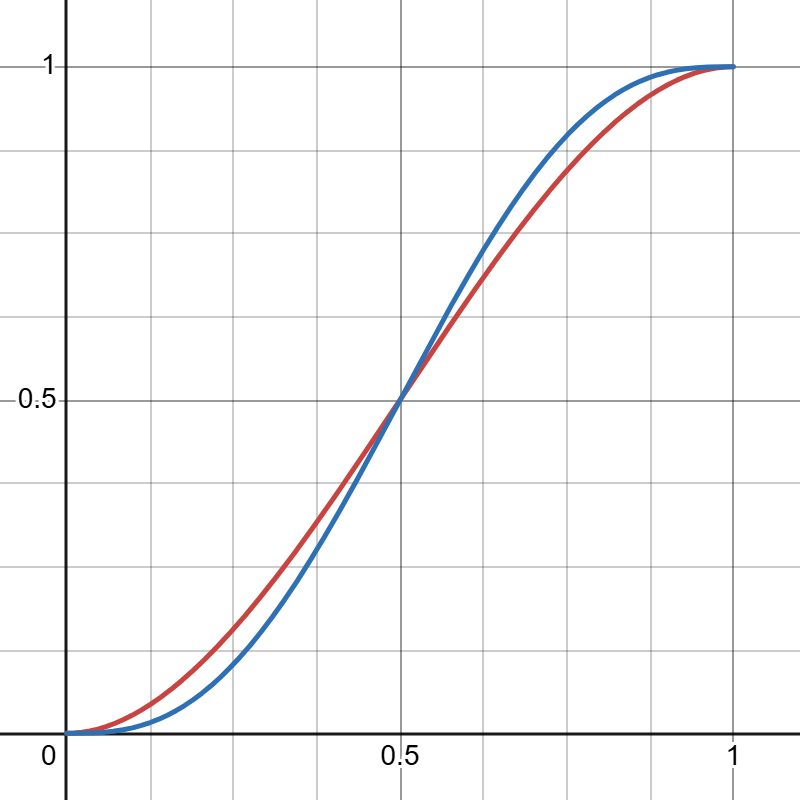
\includegraphics[width=0.75\textwidth]{smoothstep.png}
    \caption
    {
        The plot shows the third-order smoothstep function (red curve) and the fifth-order smoothstep function
        (blue curve). Both functions interpolate smoothly between 0 and 1 over the domain $[0,1]$ and has a 
        rotational symmetry at $(0.5,0.5)$, but the order-5 smoothstep function has a flatter slope at endpoints,
        resulting in smoother interpolation. Both functions were graphed using the Desmos Graphing Calculator 
        (https://www.desmos.com/calculator). 
    }
    \label{fig:smoothstep}
\end{figure}